\section{Comment on a concue notre probleme}
    % \begin{itemize}
    %     \item On a pris l'interaction des forces totale sur chaque particule par la fonction dans l'article `Cheerios effect'
    %     \item et de ca on deduis la force que reagis a chaque cheerios pour un pas de temps 
    %     \item Check si il ya des collisions ou pas et si il ya on change les proprietes des cheerios par rapport aux collisions
    %     \item De la force en utilisant l'integration de verlet et le principe fondamentale de la dynamique somme forces = derive (masse*vitesse) on peux changer les positions des cheerios
    % \end{itemize}
    Pour nos calculs pour la force de interaction des objets-bords et objet-objet on a utilise lequation\ref{eq:ForceInteraction}. Le seul probleme avec cela on a besoin de savoir langle de contact de lobjet et du bords. On sais que le verre a un angle de contact de 45° et le plastic un angle contact de 0° cest avec ceci que on a decide langle de contact de nos bords. Et pour nos objets flottants on a utilise 
    \cite{lattice_boltzmann_caplilary_interaction} 
    Voici un diagramme du fonctionnement de notre algorithme (\ref{diag:algorithme}).
    TODO DANS LE GRAPH AJOUTER POUR TOUT LES OBJETS ENTRE POURCHAQUEPASDETEMPS ET COLLISION?
    \begin{figure}[H]
        \centering
        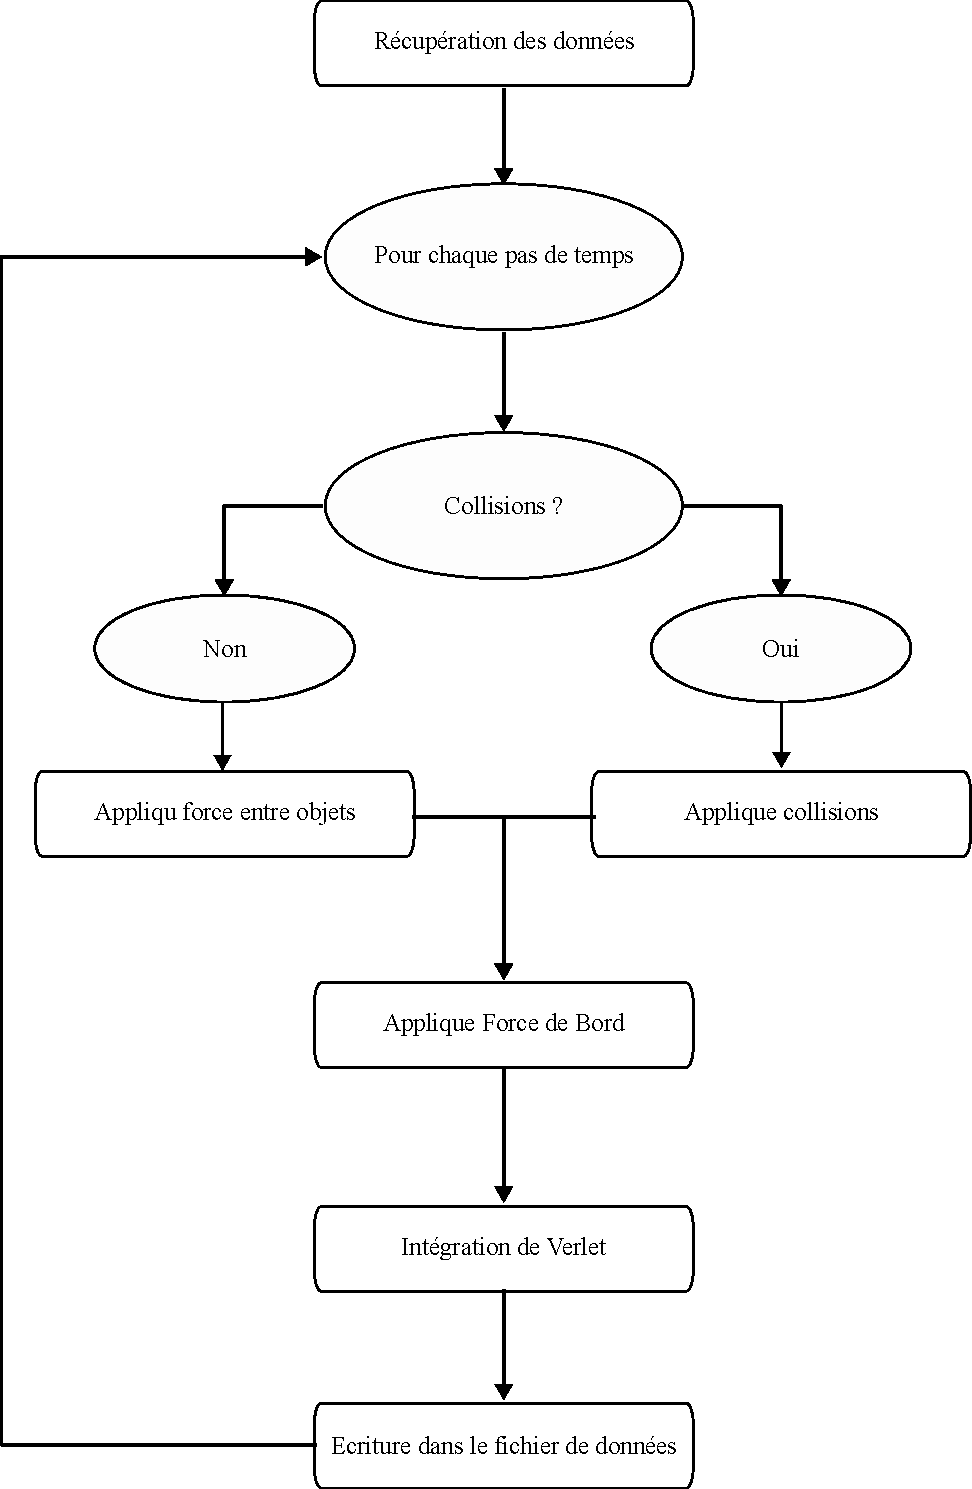
\includegraphics[width=0.45\textwidth]{Diagramme.pdf}
        \caption{Diagramme de notre algorithme}
        \label{diag:algorithme}
    \end{figure} 

    Nous avons essayé d'être le plus efficace dans notre programme et de limiter le nombre d'itération. Les données initiales sont à mettre dans un fichier texte, les données finales sont également mises dans un fichier texte. Ce dernier est lu par un script Python afin de créer l'animation avec matplotlib et sa classe \textit{animate}. Pour représenter nos objets nous utilisons la classe \textit{circle} de matplotlib également. Cela nous permet de définir des cercles avec des rayons précis.
    
\section{Les choses a ameliorer}
    \begin{itemize}
        \item Code en $O(NT\,n^2)$ et peux etre ameliorer en $O(NT\, n\log n)$ en faisant le calcul de collisions plus inteligament a la place de une recherche exasthive et en calculant une seule fois le \textit{millieu} des forces de chaque particule pour avoir un centre de atraction et comme ca on calcule le centre de attraction regarde si on a des collisions ou pas et a la fin ajoute les forces du bords a chaque particule
        \item pour linstant on utilise les equations \textit{aproximatives} on peux les essayer de les resoudres sans approximations en utilisant laproximation de Nicholson(fine difference method)
        \item le code marche seulement pour les objets ronds faux ajouter une facon plus complexe pour plus de objets
    \end{itemize}
\section*{Conclusion}
